\item \textbf{{[}ALVL/9597/2016/P1/Q3{]} }

A binary tree Abstract Data Type (ADT) has commands to create a new
tree, add unique data items to the tree and print the tree.

The sequence of commands: 

\noindent %
\noindent\begin{minipage}[t]{1\columnwidth}%
\texttt{CreateNewTree }

\texttt{AddToTree(\textquotedbl Dave\textquotedbl ) }

\texttt{AddToTree(\textquotedbl Fred\textquotedbl ) }

\texttt{AddToTree(\textquotedbl Ed\textquotedbl ) }

\texttt{AddToTree(\textquotedbl Greg\textquotedbl ) }

\texttt{AddToTree(\textquotedbl Bob\textquotedbl ) }

\texttt{AddToTree(\textquotedbl Cid\textquotedbl ) }

\texttt{AddToTree(\textquotedbl Ali\textquotedbl )}%
\end{minipage}

would create the following binary tree:
\begin{center}
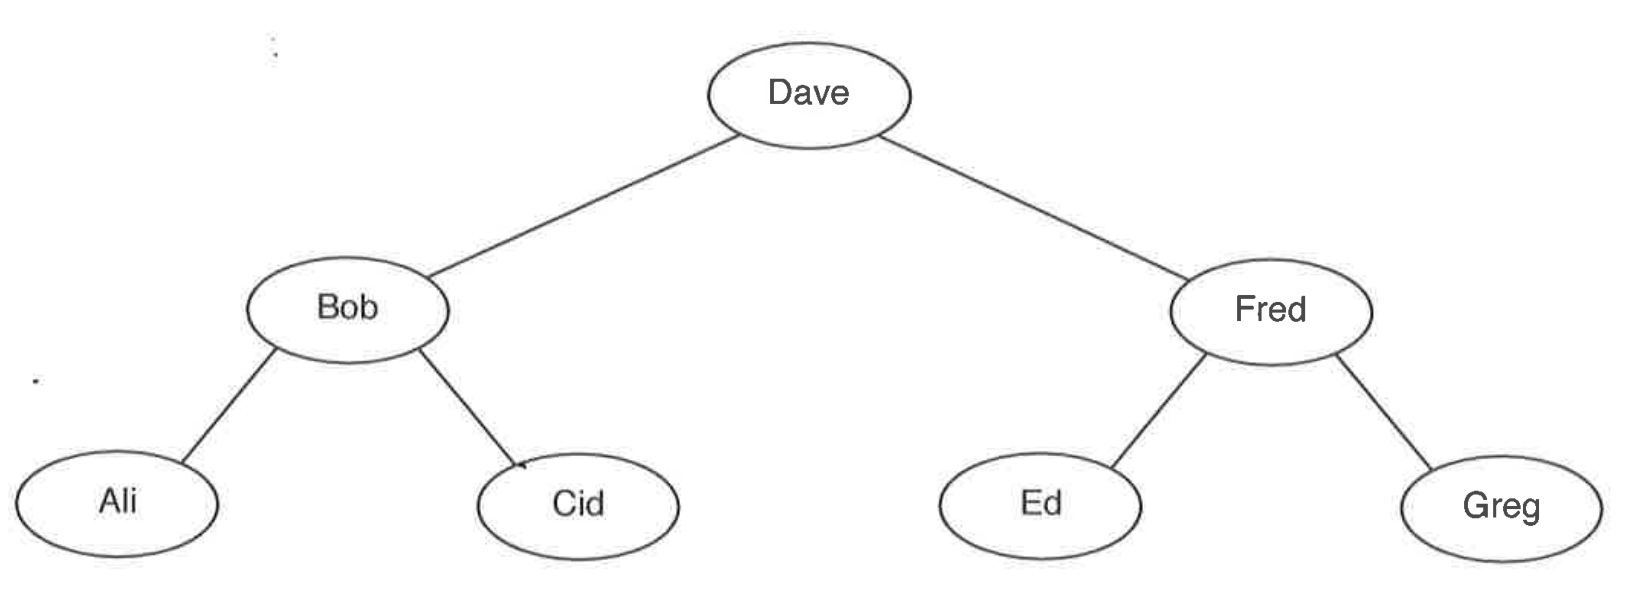
\includegraphics[width=0.5\paperwidth]{C:/Users/Admin/Desktop/Github/question_bank/static/img/9597-ALVL-2016-P1-Q3}
\par\end{center}

The program to implement this ADT will use the classes \texttt{Tree}
and \texttt{Node} designed as follows:
\begin{center}
\begin{tabular}{|l|}
\hline 
\texttt{\hspace{0.25\columnwidth}Tree}\tabularnewline
\hline 
\texttt{tree : ARRAY OF Node}\tabularnewline
\texttt{root : INTEGER}\tabularnewline
\tabularnewline
\hline 
\texttt{constructor()}\tabularnewline
\texttt{add(newItem)}\tabularnewline
\texttt{print() }\tabularnewline
\tabularnewline
\tabularnewline
\tabularnewline
\tabularnewline
\tabularnewline
\hline 
\end{tabular}%
\begin{tabular}{|l|}
\hline 
\hspace{0.25\columnwidth}\texttt{Node}\tabularnewline
\hline 
\texttt{data : STRING}\tabularnewline
\texttt{leftPtr : INTEGER}\tabularnewline
\texttt{rightPtr : INTEGER}\tabularnewline
\hline 
\texttt{constructor()}\tabularnewline
\texttt{setData(s : STRING)}\tabularnewline
\texttt{setLeftPtr(x : INTEGER)}\tabularnewline
\texttt{setRightPtr(y : INTEGER)}\tabularnewline
\texttt{getData() : STRING}\tabularnewline
\texttt{summary() : STRING}\tabularnewline
\texttt{getLeftPtr() : INTEGER}\tabularnewline
\texttt{getRightPtr() : INTEGER}\tabularnewline
\hline 
\end{tabular}
\par\end{center}

The program code must:
\begin{itemize}
\item Create a new tree, which has: 
\begin{itemize}
\item no nodes 
\item the root set to -1 
\end{itemize}
\item Use the root as a pointer to the first node in the tree 
\item Add a new node to the tree in the appropriate position 
\item Use the \texttt{print()} method to output, for each node, in array
order: 
\begin{itemize}
\item the data item 
\item the left pointer 
\item the right pointer. 
\end{itemize}
\end{itemize}

\subsubsection*{Task 3.1}

Write program code to define the classes \texttt{Tree} and \texttt{Node}. 

\subsubsection*{Evidence 6}

Your program code. \hfill{}{[}30{]}

\subsubsection*{Task 3.2}

The program is to be tested. 

Write a sequence of program statements to: 
\begin{itemize}
\item Create a tree 
\item Add the data items shown in the original list of ADT commands 
\item Print the array contents. 
\end{itemize}
Execute your program to test it. 

\subsubsection*{Evidence 7}

Your program code. 

Screenshot of test run.\hfill{} {[}3{]}

\subsubsection*{Task 3.3}

A method \texttt{inOrderTraversal()} is to be added, which outputs
the data stored in the tree in alphabetical order. 

Write program code to: 
\begin{itemize}
\item Implement this method 
\item Test the program code with the data from Task 3.2. 
\end{itemize}

\subsubsection*{Evidence 8}

Your program code. 

Screenshot of test run. \hfill{}{[}7{]}